\chapter{Supervoxel Segmentation and Superpixel Segmentation using Depth}
\label{chapter:superpixel-segmentation-depth}

The focus of this thesis is the integration of depth information into \textbf{SEEDS} \cite{VanDenBerghBoixRoigCapitaniVanGool:2012} as we believe that depth may serve as additional cue to identify object boundaries and improve the generated superpixel segmentation. Some of the superpixel algorithms discussed in section \ref{section:related-work-superpixel-segmentation} can easily be extended to use depth information, for example \textbf{CRS} \cite{ConradMertzMester:2013} and \textbf{SLIC} \cite{AchantaShajiSmithLucchiFuaSuesstrunk:2010}. Graph based approaches can also be extended to use depth information by adapting the weights accordingly, for example \textbf{ERS} \cite{LiuTuzelRamalingamChellappa:2011} and \textbf{PB} \cite{ZhangHartleyMashfordBurn:2011}. An extension of \textbf{SLIC} based on depth is discussed in the following section. However, there are more sophisticated approaches available: \textbf{DASP} \cite{WeikersdorferGossowBeetz:2012} places the initial superpixel centers depending on the depth, and with \textbf{VCCS} \cite{PaponAbramovSchoelerWoergoetter:2013}, Papon \etal provide an approach able to oversegment point clouds. We revisit both approaches in detail as they will serve as additional baselines and present state-of-the-art algorithms using depth as an integral component.

\section{SLIC using Depth Information}
\label{section:superpixel-segmentation-depth-slic3d}

\textbf{SLIC} is built around a distance function $d(x_n, S_j)$ as defined in equation \eqref{eq:superpixel-segmentation-slic-distance}. As this distance already uses pixel coordinates, we can add an additional term to introduce depth:
\begin{align}
	\label{eq:supeprixel-segmentation-depth-slic3d-distance-depth}
	d(x_n, S_j) = \|I(x_n) - I(S_j)\|_2 + \frac{\beta}{R}\|x_n - \mu(S_j)\| + \gamma\|D(x_n) - D(S_j)\|_2
\end{align}
where $\gamma$ is an additional weighting term and $D: \ubar{W} \times \ubar{H} \rightarrow \mathbb{R}$ represents a depth image. The depth of a superpixel $S_j$ is defined as $D(S_j) = \frac{1}{|S_j|} \sum_{x_m \in S_i} D(x_m)$. This distance aims to discourage superpixels crossing boundaries including a difference in depth.

Instead of using pixel coordinates and depth as separate information, we can project the pixel coordinates $x_n$ into three-dimensional space to obtain the corresponding 3D point coordinates which we denote by $P(x_n) \in \mathbb{R}^3$. The distance in equation \eqref{eq:supeprixel-segmentation-depth-slic3d-distance-depth} changes to
\begin{align}
	\label{eq:superpixel-segmentation-depth-slic3d-distance}
	d(x_n, S_j) = \|I(x_i) - I(S_j)\|_2 + \beta \| P(x_n) - P(S_j) \|_2
\end{align}
with $P(S_j) = \frac{1}{|S_j|} \sum_{s_m \in S_j} P(x_m)$. Connectivity can still be enforced on the image plane. We implemented this variant of \textbf{SLIC}, in the following referred to as \textbf{SLIC3D}, as additional baseline.

\subsection{Discussion}

Because of \textbf{SLIC}'s good performance, we do not expect a significant increase in performance while slightly increasing the runtime due to the extended distance in equation~\eqref{eq:superpixel-segmentation-depth-slic3d-distance}. However, we are able to observe a visual difference in the generated superpixels as, depending on the value of $\beta$, \textbf{SLIC3D} enforces compactness within three dimensional space such that the superpixels appear to reflect the underlying three dimensional structure. Figure \ref{fig:superpixel-segmentation-slic3d-comparison} shows the generated superpixel segmentations of the running examples.
\begin{figure}[t]
	\centering
	\subfigure{
		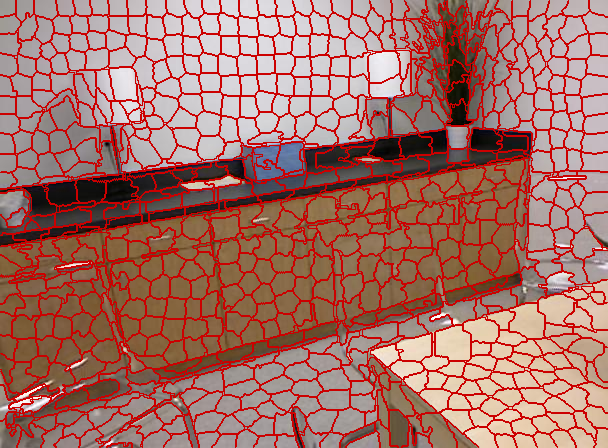
\includegraphics[scale=\scalefivenyu]{pictures/nyu-1-slic3d}
	}
	\subfigure{
		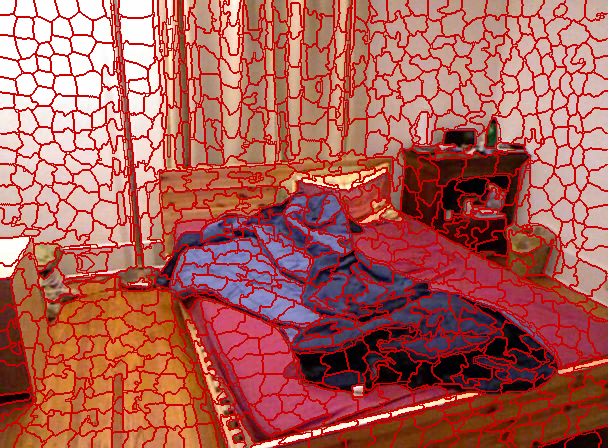
\includegraphics[scale=\scalefivenyu]{pictures/nyu-2-slic3d}
	}
	\subfigure{
		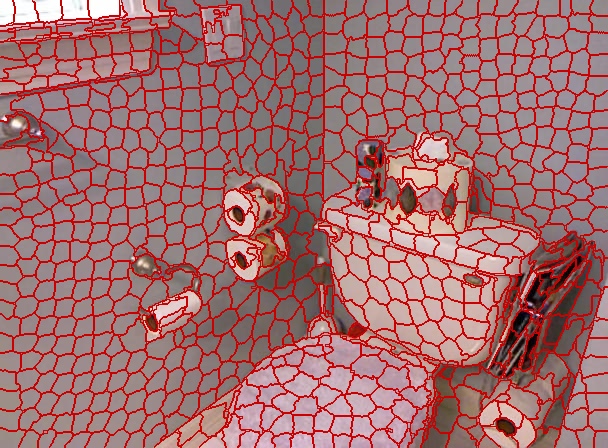
\includegraphics[scale=\scalefivenyu]{pictures/nyu-3-slic3d}
	}
	\subfigure{
		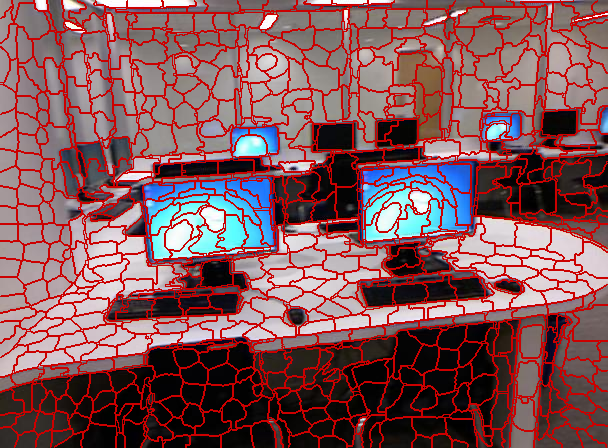
\includegraphics[scale=\scalefivenyu]{pictures/nyu-4-slic3d}
	}
	\subfigure{
		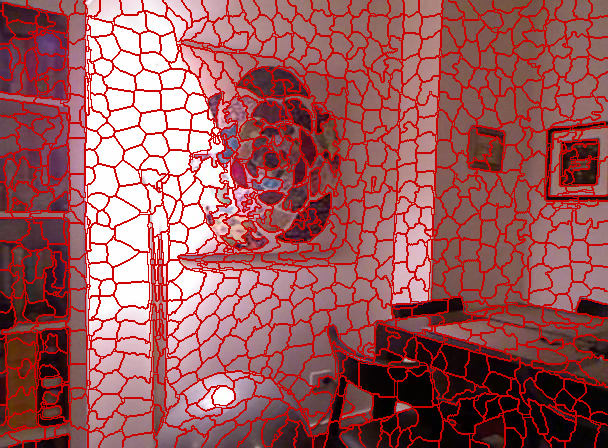
\includegraphics[scale=\scalefivenyu]{pictures/nyu-5-slic3d}
	}
	\caption[The running examples oversegmented using an extension of \textbf{SLIC} \cite{AchantaShajiSmithLucchiFuaSuesstrunk:2010} using depth information.]{Superpixel segmentations with roughly $840$ superpixels of the running examples generated using \textbf{SLIC3D}. Further examples can be found in section \ref{subsection:evaluation-comparison-qualitative} or appendix \ref{chapter:appendix-evaluation}.}
	\label{fig:superpixel-segmentation-slic3d-comparison}
\end{figure}

\section{DASP}
\label{section:superpixel-segmentation-dasp}

% TODO: add derivation of area.
% TODO: mention generalization of concept known as ASP (see GitHub)
The approach proposed by Weikersdorfer \etal \cite{WeikersdorferGossowBeetz:2012} is based on an important observation. Usually, we choose the number of superpixels such that we obtain superpixels comparable in size to the smallest objects we are interested in \cite{WeikersdorferGossowBeetz:2012}. Consequently, the density of superpixels is higher at surfaces farther away from the image plane \cite{WeikersdorferGossowBeetz:2012}, that is with increasing depth the superpixels get smaller on average. Nevertheless, we want the superpixels to be distributed uniformly on surfaces at any depth. This is achieved by defining a superpixel density on the depth image. We follow \cite{WeikersdorferGossowBeetz:2012} and consider a disk of radius $R$ centered at pixel $x_n$ in depth $D(x_n)$. Using the model of a pinhole camera \cite{ForsythPonce:2002}, the radius of this disk projected onto the image plane is given by
\begin{align}
	r(x_n) = \frac{f}{D(x_n)} R
\end{align}
where $f$ denotes the focal length of the camera. As noted in \cite{WeikersdorferGossowBeetz:2012}, this equation can only be applied in cases where the disk is parallel to the image plane. Otherwise, a projective transformation would be necessary which Weikersdorfer \etal approximate using an affine transformation. First, the gradient $\nabla D(x_n)$ of the depth image is estimated using finite differences. Then, the area of the projected disk can be expressed~as
\begin{align}
	A(x_n) = \frac{r(x_n)^2\pi}{\sqrt{\|\nabla D(x_n)\|_2^2 + 1}}
\end{align}
and the superpixel density at pixel $x_n$ is proportional to $\frac{1}{A(x_n)}$. A detailed derivation can be found in \cite{Weikersdorfer:2014}. In practice, the provided implementation of \textbf{DASP} offers several methods to sample the initial superpixel centers from this density, one of which is given by random sampling, summarized in algorithm \ref{algo:superpixel-segmentation-depth-dasp-random}.
\begin{algorithm}[t!]
	\begin{algo}{DASP (sed sampling)}{\label{algo:superpixel-segmentation-depth-dasp-random}\qinput{color image $I$, density $p(x_n) \propto \frac{1}{A(x_n)}$}\qoutput{superpixel centers $\mu(S) = \{\mu(S_1),\ldots,\mu(S_K)\}$}}
		initialize $\mu(S) = \emptyset$\\
		\qfor $n = 1$ \qto $N$\\
			$r$ \qlet $random([0, 1])$\\
			\qif $r < p(x_n)$\\
				\qthen $\mu(S)$ \qlet  $\mu(S) \cup \{x_n\}$\qfi\qrof\\
		\qreturn $\mu(S)$
	\end{algo}
	\caption[\textbf{DASP} \cite{WeikersdorferGossowBeetz:2012} randomly samples the initial superpixel centers from a custom density based on depth information.]{The easiest way to sample superpixel centers form the superpixel density $p(x_n)$ is given by random sampling. For each pixel, a number in the range $[0,1]$ is randomly chosen and compared to the probability $p(x_n)$ of $x_n$ being an initial superpixel center. For details how the desired number of superpixels is met we refer to the implementation\footnote{Available at \url{https://github.com/Danvil/dasp}.}.}
	\label{fig:superpixel-segmentation-depth-dasp-random}
\end{algorithm}
Note that the above mechanism can also be applied to custom densities or densities based on different information, see \cite{Weikersdorfer:2014} for details.

Similar to \textbf{SLIC}, the algorithm alternates between the assignment step where each pixel is assigned to the nearest superpixel and the update step where the superpixel centers are updated. The used distance is given by
\begin{align}
	\label{eq:superpixel-segmentation-depth-dasp-distance}
	d(x_n, S_j) = \|I(x_n) - I(S_j)\|_2 + \beta\|P(x_n) - P(S_j)\|_2 + \gamma \left(1 - N(x_n)^T N(S_j)\right)
\end{align}
where $\beta$ and $\gamma$ are parameters weighting the corresponding terms and $N(x_n)$ denotes the normal corresponding to pixel $x_n$ which we assume to be normalized. Again, we use $N(S_j) = \frac{1}{|S_j|} \sum_{x_m \in S_j} N(x_m)$ and the normals are estimated using depth gradients. The term $N(x_n)^T N(S_j)$ represents the cosine of the angle between the normals $N(x_n)$ and $N(S_j)$. Here, the intuition is that pixel $x_n$ and superpixel $S_j$ lie on the same planar surface if this angle is small. On the other hand, the cosine of this angle reaches zero if the normals are orthogonal to each other.

\subsection{Discussion}

In contrast to \textbf{SLIC3D}, the approach presented above not only uses 3D point coordinates and normal information but also adapts the size of superpixels according to the given depth. This way we expect to get performance comparable to superpixel algorithms like \textbf{SLIC} and \textbf{SEEDS}, however, with a lower number of superpixels. Additionally, by using normal information, \textbf{DASP} may recognize additional boundaries not apparent when using color and 3D point coordinates only. Figure \ref{fig:superpixel-segmentation-depth-dasp-comparison} shows the running examples oversegmented using \textbf{DASP}.
\begin{figure}[t]
	\centering
	\subfigure{
		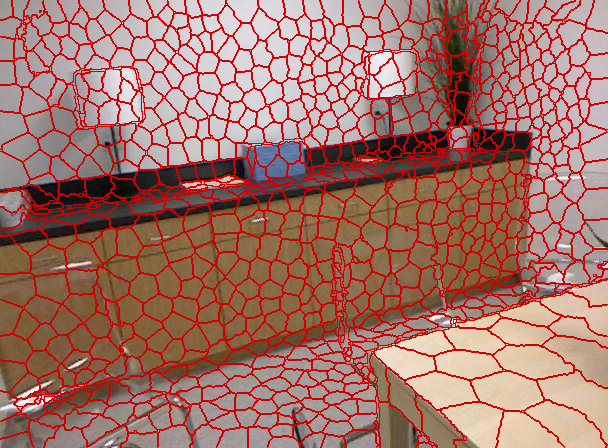
\includegraphics[scale=\scalefivenyu]{pictures/nyu-1-dasp}
	}
	\subfigure{
		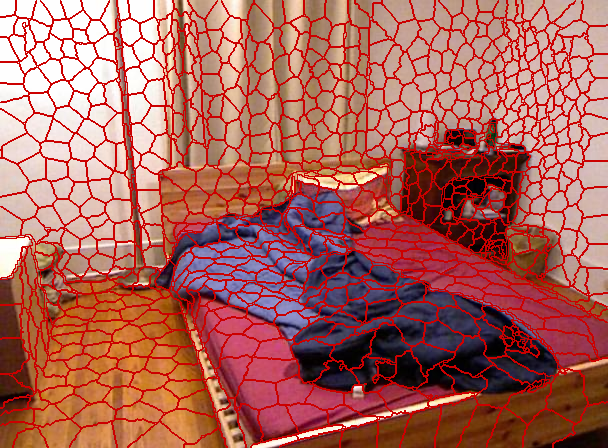
\includegraphics[scale=\scalefivenyu]{pictures/nyu-2-dasp}
	}
	\subfigure{
		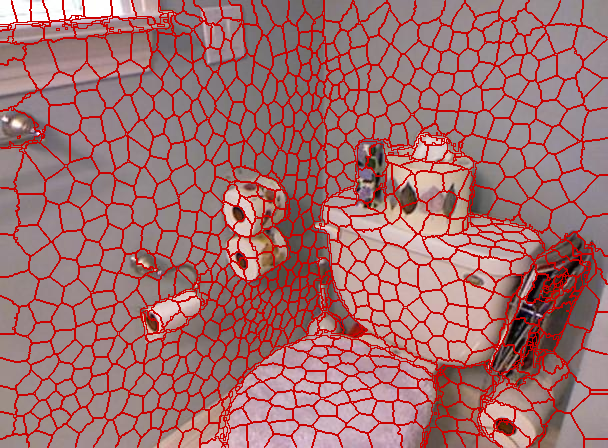
\includegraphics[scale=\scalefivenyu]{pictures/nyu-3-dasp}
	}
	\subfigure{
		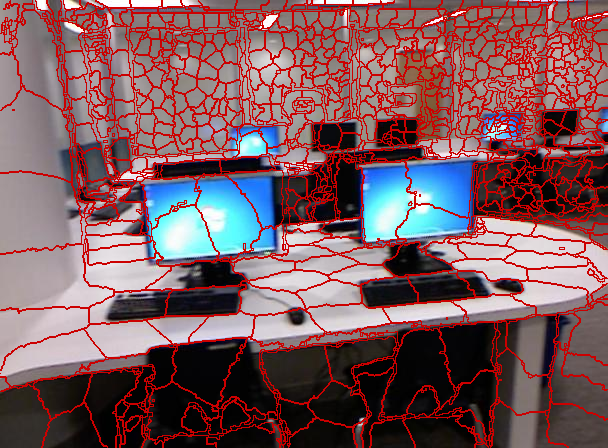
\includegraphics[scale=\scalefivenyu]{pictures/nyu-4-dasp}
	}
	\subfigure{
		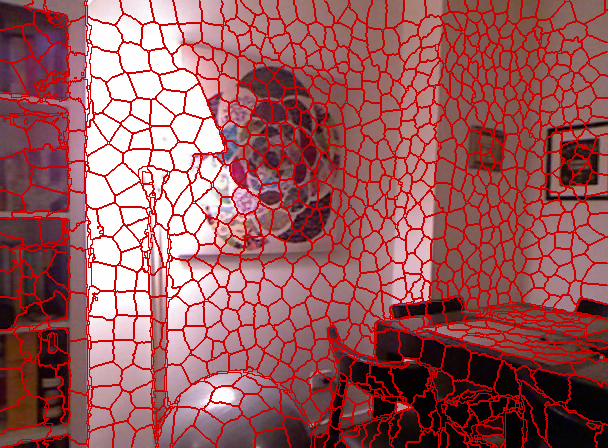
\includegraphics[scale=\scalefivenyu]{pictures/nyu-5-dasp}
	}
	\caption[Superpixel segmentations of the running examples generated by \textbf{DASP} \cite{WeikersdorferGossowBeetz:2012}.]{Superpixel segmentations with roughly $840$ superpixels of the running examples generated by \textbf{DASP}. Further examples are available in section \ref{subsection:evaluation-comparison-qualitative} and appendix \ref{chapter:appendix-evaluation}.}
	\label{fig:superpixel-segmentation-depth-dasp-comparison}
\end{figure}

\section{VCCS}
\label{section:superpixel-segmentation-depth-vccs}

% TODO: introduce background on point clouds!
% TODO: introduce different notion of S_i (set of 3D points now).
Although \textbf{VCCS} may be applied to arbitrary point clouds as for example generated from multiple RGB-D cameras or laser scans \cite{PaponAbramovSchoelerWoergoetter:2013}, we assume the point cloud to be created from a single image with corresponding depth image. Note that this results in a dense and ordered point cloud\footnote{That is, the points are accessible by their pixel coordinates within a two dimensional array.}. The point cloud is voxelized using a given voxel resolution $R_v$ such that an $26$-adjacency graph can be defined, see \cite{Rusu:2009} for details.

The idea of \textbf{VCCS} is similar to \textbf{SLIC} in that it performs local $K$-means clustering within the voxelized point cloud. However, \textbf{VCCS} ensures connectivity by applying breadth-first search as basis for clustering. After placing supervoxel centers at a regular grid with step size\footnote{Note that this step size is applied in three dimensional space.} $R$, also called supervoxel resolution\footnote{Actually, Papon \etal \cite{PaponAbramovSchoelerWoergoetter:2013} call $R$ seed resolution where a seed corresponds to a supervoxel center. This naming is often used for superpixel centers as well \cite{AchantaShajiSmithLucchiFuaSuesstrunk:2010}.}, we first need to remove supervoxel centers which have no voxels in their immediate neighborhood. If a given supervoxel center would lie on a planar surface, then the following equation yields the number of voxels within a specified search radius $R_s$:
\begin{align}
	\frac{R_s^2 \pi}{R_v^2}
\end{align}
where $R_v^2$ describes the ground area of a single voxel. All supervoxel centers having less voxels in the sphere of radius $R_s$ are discarded (see the implementation in the Point Cloud Library\footnote{The Point Cloud Library, implemented in C++, is mainly aimed to provide state-of-the-art computer vision algorithms running on point clouds: \url{http://pointclouds.org/}.} \cite{RusuCousins:2011} for details). Afterwards, the supervoxel centers are moved to low gradient magnitude positions similar to \textbf{SLIC}.% Furthermore, the supervoxel centers are moved to the mean position within a local neighborhood.

According to \cite{PaponAbramovSchoelerWoergoetter:2013}, \textbf{VCCS} performs clustering in a $39$ dimensional space comprising color, 3D point coordinates and Fast Point Feature Histograms \cite{RusuBlodowBeetz:2009}, short FPFH. However, the implementation available as part of the Point Cloud Library suggests that instead of FPFH features, point normals are used. Additionally, our experiments suggest that using FPFH features is quite expensive regarding runtime. Thus, we focus on the version as provided by the Point Cloud Library. The used distance function is given by
\begin{align}
	\label{eq:superpixel-segmentation-depth-vccs-distance}
	d(x_n, S_j) = \|I(x_n) - I(S_j)\|_2 + \beta\|P(x_n) - P(S_j)\|_2 + \gamma \left(1 - N(x_n)^T N(S_j)\right)
\end{align}
where $\beta$ and $\gamma$ are parameters weighting the spatial and normal terms.

\begin{algorithm}[t]
	\begin{algo}{VCCS}{\label{algo:superpixel-segmentation-depth-vccs}\qinput{voxelized point cloud, supervoxel resolution $R$, search radius $R_s$}\qoutput{superpixel segmentation $S$}}
		place supervoxel centers on a regular grid with step size $R$\\
		discard unnecessary supervoxel centers based on the search radius $R_s$\\		
		move supervoxel centers to low gradient magnitude positions\\
		%\qcom{Eventually, move supervoxel centers to mean position within local neighborhood}\\
		\qfor $t = 1$ \qto $T$ \qcom{$T$ is the maximum depth.}\\
			\qfor $k = 1$ \qto $K$\\
				perform one step breadth first search for supervoxel $S_k$\\
				update supervoxel center\qrof\qrof\\
		derive superpixel segmentation $S$ by backprojecting the supervoxels\\
		\qreturn $S$
	\end{algo}
	\caption[The supervoxel algorithm \textbf{VCCS} \cite{PaponAbramovSchoelerWoergoetter:2013}.]{\textbf{VCCS} uses $K$-means clustering based on breadth-first search beginning at the supervoxel centers to assign each voxel to a supervoxel. This way, \textbf{VCCS} ensures that the supervoxels represent connected components within the $26$-adjacency graph derived from the voxelized point cloud. The below algorithm can easily be adapted to return a supervoxel segmentation instead of a superpixel segmentation.}
	\label{fig:superpixel-segmentation-depth-vccs-breadth-first}
\end{algorithm}
The clustering process is different to the local $K$-means clustering used by \textbf{SLIC} in that it implements a breadth-first search beginning at the supervoxel centers. As for \textbf{SLIC}, the pixels being of interest for a particular supervoxel $S_j$ are limited by the maximum depth $T$ of the breadth-first search. In practice, the maximum depth $T$ is set to
\begin{align}
	T = 1.8 \cdot \frac{R}{R_v}.
\end{align}
\textbf{VCCS} is, slightly simplified, described in algorithm \ref{algo:superpixel-segmentation-depth-vccs}.

\subsection{Discussion}

While the approaches discussed in section \ref{section:superpixel-segmentation-depth-slic3d} and \ref{section:superpixel-segmentation-dasp} generate superpixel segmentations using depth as additional cue, \textbf{VCCS} creates supervoxels directly in three dimensional space. This is advantageous when considering input from multiple RGB-D cameras describing the same scene or laser scans \cite{PaponAbramovSchoelerWoergoetter:2013}. Furthermore, the algorithm can be applied to unordered point clouds. Additionally, in contrast to \textbf{SLIC}, \textbf{VCCS} does not need to enforce connectivity afterwards.

On the other hand, being dependent on a point cloud can also have major disadvantages when aiming to oversegment images for which depth information is available separately. For example \textbf{SLIC3D} or \textbf{DASP} can easily be applied to images with incomplete depth information by falling back to a color only mode. As we discuss in chapter \ref{chapter:datasets}, this is often the case when grabbing raw images from RGB-D cameras like the Microsoft Kinect. In such a case we are not able to generate a complete point cloud such that \textbf{VCCS} cannot be applied to the whole image. However, note that these considerations differ depending on the application. Furthermore, we note that the comparison of superpixel algorithms with supervoxel algorithms is difficult by design.

As the distance used for clustering is equal to the distance used by \textbf{DASP}, we cannot expect to observe increased performance due to different features. However, in contrast to \textbf{SLIC3D} and \textbf{DASP}, \textbf{VCCS} avoids stray labels and respects the underlying three dimensional surface directly by oversegmenting a point cloud in the form of a $26$-adjacency graph. Although \textbf{SLIC3D} and \textbf{DASP} would be able to detect boundaries within the depth image, depending on the parameter $\beta$, these boundaries can also be ignored. Due to the breadth-first search utilized by \textbf{VCCS} such cases are handled automatically. Overall, we expect improved performance for a lower number of superpixels when compared to other approaches. \textbf{VCCS} applied to the running examples is shown in figure \ref{fig:superpixel-segmentation-depth-vccs-comparison}.

% Beneath the above difficulties, there are further aspects to discuss concerning the algorithm and its implementation. First of all, \textbf{VCCS} is available as part of the Point Cloud Library \cite{Rusu:2009}. However, the implementation differs from the proposed algorithm in \cite{PaponAbramovSchoelerWoergoetter:2013} in that FPFH features are not used for clustering. Instead, a distance similar to the one used by \textbf{DASP} is utilized. Nevertheless, \textbf{VCCS} has the advantage that it avoids stray labels as known from \textbf{SLIC}. Overall, we expect not to get increased performance because of the different features used but rather because of a different initialization of the supervoxel centers and clustering directly within a point cloud. As using \textbf{DASP} this may result in performance comparable to superpixel algorithms not using depth information while generating less supervoxels. \textbf{VCCS} applied to our running examples can be seen in figure \ref{fig:superpixel-segmentation-depth-vccs-comparison}.
\begin{figure}[t]
	\centering
	\subfigure{
		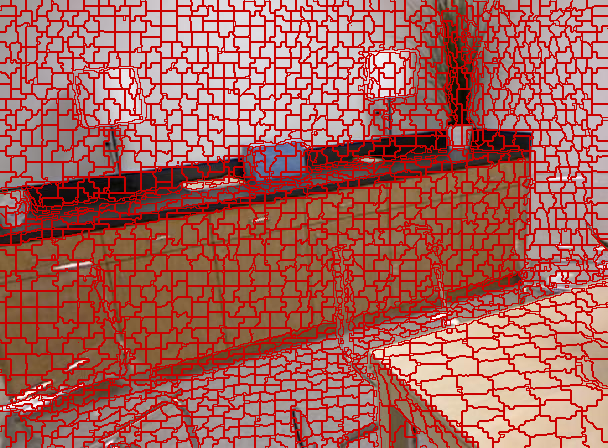
\includegraphics[scale=\scalefivenyu]{pictures/nyu-1-vccs}
	}
	\subfigure{
		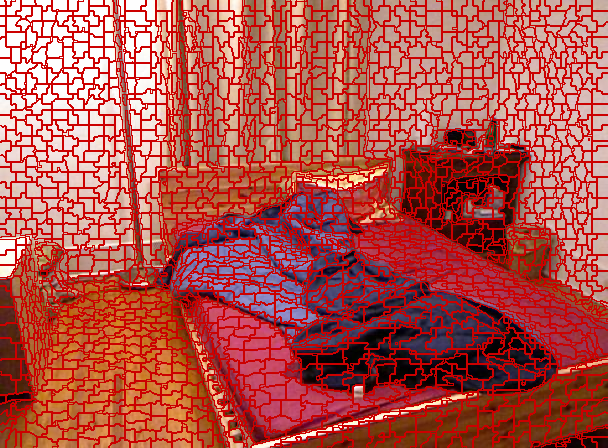
\includegraphics[scale=\scalefivenyu]{pictures/nyu-2-vccs}
	}
	\subfigure{
		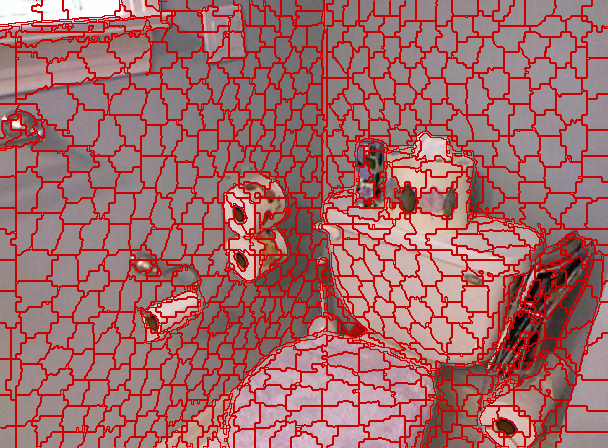
\includegraphics[scale=\scalefivenyu]{pictures/nyu-3-vccs}
	}
	\subfigure{
		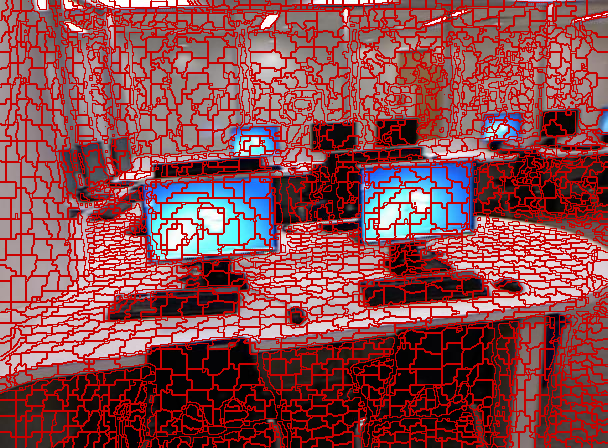
\includegraphics[scale=\scalefivenyu]{pictures/nyu-4-vccs}
	}
	\subfigure{
		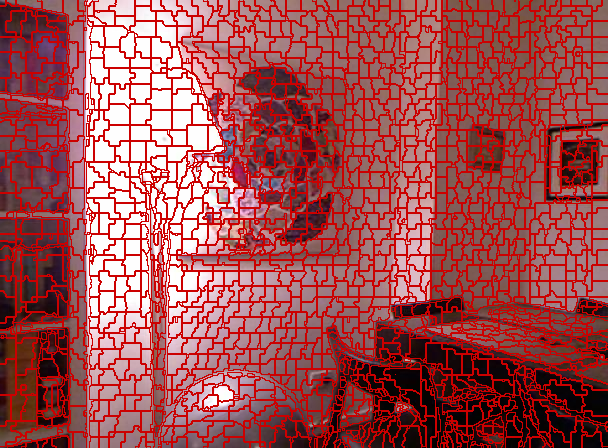
\includegraphics[scale=\scalefivenyu]{pictures/nyu-5-vccs}
	}
%	\subfigure[] {
%		\label{subfig:superpixel-segmentation-vccs-comparison-cloud-1}
%		\includegraphics[scale=0.145]{pictures/nyu-1-vccs-cloud}
%	}
%	\subfigure[] {
%		\label{subfig:superpixel-segmentation-vccs-comparison-cloud-2}
%		\includegraphics[scale=0.155]{pictures/nyu-2-vccs-cloud}
%	}
%	\subfigure[] {
%		\label{subfig:superpixel-segmentation-vccs-comparison-cloud-3}
%		\includegraphics[scale=0.145]{pictures/nyu-3-vccs-cloud}
%	}
	\caption[The running examples oversegmented using \textbf{VCCS} \cite{PaponAbramovSchoelerWoergoetter:2013}.]{The running examples oversegmented into roughly $840$ superpixels using \textbf{VCCS}. Further examples can be found in section \ref{subsection:evaluation-comparison-qualitative} and appendix \ref{chapter:appendix-evaluation}.}
	\label{fig:superpixel-segmentation-depth-vccs-comparison}
\end{figure}